\label{referencial}

Neste Capítulo apresentamos os conceitos necessários para o entendimento deste trabalho. 

\section{Engenharia de Software}

 A partir do início da década de 1940, os computadores eram criados com um fim específico, rodando apenas para o fim específico ao qual foi projetado, como por exemplo o Colossus, primeira máquina computacional criada  por Alan Turing que se tem registrado, com o fim de decifrar mensagens criptografadas enviadas pelos alemães \cite{colossus}. Esta era uma época onde máquinas eram construídas para realizar apenas um único propósito computacional programável, com uma única tarefa a ser executada desde o princípio de sua existência. Pouco tempo após, vimos a criação dos primeiros computadores que permitiam rodar mais do que um único programa, lendo a partir de cartões perfurados o que o computador deveria executar ou qual poderia ser uma resposta esperada, conforme descrito por Dijsktra \cite{Humble}. 
 
 Com o passar do tempo, miniaturização, modernização e a popularização dos computadores, podendo estes serem usados dentro de firmas empresariais, órgãos governamentais, universidades e até mesmo em casas (apesar dos proibitivos preços), fazendo assim com que novas gamas de capacidades fossem dadas aos computadores. Com isto, naturalmente novos softwares e linguagens de programação foram sendo criados, e trazendo consigo o início da popularização das áreas de desenvolvimento de software e como estas poderiam produzir um produto de qualidade com um tempo razoável e um custo factível. Porém, o que se viam era exatamente o contrário, onde durante a produção destes aplicativos víamos projetos estourando o orçamento e o tempo previsto, uma qualidade bem aquém do esperado, não atendiam ao usuário final devidamente e de custosa manutenção e verificação dos códigos, conforme foi constado por Naur e Randell na conferência do comitê de ciência da \acrshort{OTAN}\cite{NATO}. A partir daí, verificando que alguns métodos derivados da administração poderiam funcionar também na produção de software, vemos o nascimento de métodos formais para o auxílio na construção de tais ferramentas de uso computacional. E daí, temos a criação do desenvolvimento da área de Engenharia de software, também citada pela primeira vez na conferência do comitê de ciência da \acrshort{OTAN}\cite{NATO}.

Engenharia de software é o processo que foca nas áreas de planejamento, desenvolvimento e entrega dos sistemas de software. É com este tipo de metodologia que conseguimos estimar de maneira mais apurada formas de como desenvolver o sistema, estimar prazos, recursos e até mesmo espaços para melhora durante e após a conclusão do projeto. A engenharia de software nasceu da necessidade de entregar ao cliente uma maior garantia de qualidade, sem deixar de lado a preocupação com prazos, estes cada vez mais curtos perante as demandas que o mundo e sua evolução tecnológica tem exigido de acordo Sommerville\cite{Sommerville07}. Para Pressman \cite{pressman}, a Engenharia de Software envolve processos, métodos e ferramentas que permitem aos profissionais
construir softwares bem desenvolvidos. Para Wazlawick \cite{wazlawick}, a Engenharia de Software é olhada como o meio de estudo, criação e otimização de processos para o desenvolvimento de software, onde as atividades essenciais de um engenheiro de software envolve a especificação do software, seu desenvolvimento, validação e sua evolução.

Uma dos motivos que a Engenharia de Software se tornou algo extremamente relevante é a crescente necessidade da sociedade e dos indivíduos e como se relacionam com os sistemas de software, onde estes necessitam ser pensados e projetados com a maior excelência possível para se ter segurança, performance e possibilidade de manutenção. A partir de um olhar no aspecto econômico, um outro motivo é que, a longo prazo, se torna mais barato utilizar técnicas e métodos de Engenharia de Software ao invés de projetar sistemas sem a padronização demandada sem estas técnicas e métodos, já que para a maior parte dos de sistemas de software, boa parte dos custos estão ligados as modificações realizadas no software após sua implantação, quando este já se encontra em produção \cite{Sommerville07}.

Em suma, a Engenharia de Software é uma disciplina que envolve diversas áreas, à exemplo: processos de software, desenvolvimento ágil, engenharia de requisitos, testes
de software, evolução de software e segurança. Assim, dada a importância crucial dos sistemas de software para todos os aspectos da nossa sociedade atual.

\subsection{Engenharia de Requisitos}

A engenharia de requisitos (ou especificação de software) é a área responsável por entender e decidir quais serão as requisições necessárias ao sistema solicitado e verificar os impedimentos relacionados ao desenvolvimento e operação do sistema. Costuma ser um estágio crítico do processo de criação de um software, pois uma vez mal desenhado e com erros nesta fase, mais a frente no projeto, implantação e manutenção do sistema problemas serão comuns de aparecerem, segundo Sommerville \cite{Sommerville07}. Para Pressman \cite{pressman}, é a área que engloba as tarefas e técnicas que guiam a uma noção mais precisa possível dos requisitos, sendo esta uma das ações principais da Engenharia de Software. 

Esta etapa existe com o propósito de criar uma documentação de requisitos acordados onde cria a especificação de um sistema que possa atender às necessidades dos clientes atendidos para o desenvolvimento do software. Usualmente, os requisitos são postos para seus clientes e usuários finais em um nível mais alto, sem grandes detalhes técnicos, enquanto para os desenvolvedores é essencial que os detalhes técnicos sejam muito bem apresentados \cite{Sommerville07}.

De acordo Sommerville \cite{Sommerville07}, são quatro níveis principais do processo de engenharia de requisitos, conforme apresentado na Figura \ref{fig:eng_req}, os quais são:

\begin{enumerate}
    \item \textit{Estudo de viabilidade}: Realiza-se uma aproximação a respeito a possibilidade de se cumprir com as requisições do usuário em questão, valendo-se de tecnologias contemporâneas, seja a nível de software ou de hardware. Esse estudo leva em conta se o sistema a ser criado será lucrativo sobre uma posição de negócio e se o mesmo pode ser construído sob condições financeiras limitadas. Um estudo de viabilidade deve ser algo sem grandes custos e de rápida conclusão, onde o resultado culmina na decisão ou não de continuar com a possibilidade de um estudo mais detalhado.
    
    \item \textit{Elicitação e análise de requisitos}: Esta é a parte do processo onde se inicia a formação mais aprofundada dos requisitos do sistema por meio da análise de outros sistemas existentes, além de debates com os potenciais clientes/usuários e compradores, verificação de tarefas e outras etapas. É nesta parte onde a criação de protótipos ou modelos de sistemas são feitos para ajudar a elucidar o sistema a ser criado.
    
    \item \textit{Especificação de requisitos}: A etapa de ação de tradução dos dados e informações coletados durante a etapa de análise de uma documentação que detalha o conjunto de requisitos. Geralmente, são dois os tipos de requisitos que podem ser inseridos nesta documentação. A parte onde o cliente menciona o que deseja criar para o seu produto de forma mais geral e sem a profundidade técnica, mais voltada para o objeto de desejo de uso é chamada de requisitos de usuário, enquanto a parte onde há um maior detalhamento na descrição técnica a ser fornecido ao usuário é chamado de requisitos de sistema.
    
    \item \textit{Validação de requisitos}: Esta etapa é onde verificamos se o sistema está consistente, completo e de acordo com a realidade, onde não por acaso se descobrem os principais erros e a documentação deve ser alterada de forma a visar a correção destes problemas que foram mapeados durante esta etapa.
\end{enumerate}

\begin{figure}
    \centering
    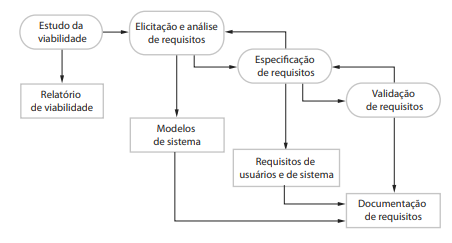
\includegraphics{img/eng_req.png}
    \caption{Gráfico do processo de engenharia de requisitos} \cite{Sommerville07}
    \label{fig:eng_req}
\end{figure}


De acordo com Sommerville \cite{Sommerville07}, as atividades decorrentes do processo não são realizadas de forma linear e sequencial. Até alcançar a fase de entrega final, várias iterações novas são pensadas para novas definições, especificações e revisões dos requisitos, mostrando que tais etapas são de certa forma ligadas em cadeia. Nos modelos ágeis de desenvolvimento, como o \textit{Extreme Programming}, os requisitos são criados, desenvolvidos e entregues de forma a incrementar sempre a iteração anterior de acordo as necessidades básicas e essenciais do usuário, enquanto o processo de elicitação de requisitos é feita pelos usuários que estão testando a ferramenta juntamente com o time de desenvolvedores.
 
 De acordo com Fleming \cite{cmmi}, a área de engenharia de requisitos tem em mente três pontos em específico: 1) a área de desenvolvimento de requisitos do cliente fornece um conjunto de requisitos por parte do usuário que vão fornecer os requisitos para o desenvolvimento dos requisitos do produto; 2) a área de desenvolvimento de requisitos de produto fornece a partir dos requisitos dos componentes do produto o design a ser usado nos produtos ou em seus componentes; e 3) a análise e a validação dos requisitos fornece a necessidade de análise do usuário, produto e dos componentes do produto para definir, extrair e entender os requerimentos. As práticas em específico do terceiro ponto levam a suportar as práticas em especificações nos dois primeiros pontos em específico. O processo associado com a área de engenharia de requisitos e correlatas podem servir integralmente para a área técnica responsável, a qual pode interagir de forma recursiva, contribuindo também na agilidade do desenvolvimento do produto para o usuário final.
 
 \subsection{Elicitação de Requisitos}
 
 Uma das primeiras atividades a serem realizadas nos processos de Engenharia de Requisitos (RE) é a elicitação de requisitos, onde esta se passa pelos processos de aprendizado, imersão e descoberta de necessidades \cite{Hadar}. Esta área está diretamente ligada as origens dos requisitos do sistema e como os responsáveis pela engenharia de software conseguem coletá-los \cite{SWEBOK2014}. Para tanto, os profissionais da área, junto aos clientes e usuários finais do sistema em criação, trabalham de forma a obter insumos e dados a respeito o domínio da aplicação, os serviços a serem ofertados pelo sistema, como ele se desempenha, quais as limitações de hardware e assim por diante, de acordo Sommerville \cite{Sommerville07}.

Essa atividade é realizada de forma puramente humana, onde os stakeholders são identificados e, a partir daí, o relacionamento entre equipe de desenvolvimento e cliente são consolidadas \cite{SWEBOK2014}. Essa atividade passa pelo envolvimento de diversos tipos de perfis dentro de uma organização, como por exemplo os próprios stakeholders, onde também se inserem os usuários finais que irão usar o sistema e/ou qualquer outra pessoa que seja afetada com este uso, de acordo Sommerville \cite{Sommerville07}.

A elicitação tem como foco a identificação do problema, proposição de elementos para a solução, a negociação de abordagens distintas e a especificação de um conjunto primitivo de requisitos do produto em um ambiente que seja apto para o alcance deste objetivo \cite{pressman}. Um dos aspectos principais para uma elicitação de requisitos ser alcançado com sucesso é a fácil e eficiente comunicação entre os diversos stakeholders \cite{SWEBOK2014}.

Para tanto, é necessário uma coleção de modelos que seja consistente nos mais variados níveis de abstração, visando facilitar a comunicação entre os usuários do sistema (stakeholders) e os engenheiros de software \cite{SWEBOK2014}. Temos a disposição vários tipos de modelos de elicitação e análise de requisitos, onde para cada organização temos a sua versão ou instância que dependem de fatores ambientais locais, como por exemplo o nível de conhecimento do pessoal, a espécie de sistema a ser criado, quais normas serão usadas, entre outros \cite{Sommerville07}. 
 
\section{Desenvolvimento Ágil de Software}

Idealizado em 2001 em uma carta pública divulgada na internet, o manifesto ágil, criado por Kent et al. \cite{agilemanifesto} veio para se transformar em uma revolução na forma de transformar os projetos para criação de produtos baseados em programação. Com o lema de valorizar indivíduos e interações, software em funcionamento, colaboração com o cliente e responder as mudanças, a mudança de paradigma que o manifesto trouxe na produção de software foi imediata, sendo estes princípios derivados a partir do modelo \textit{Extreme Programming}, também conhecido como \acrshort{XP}. Com este modelo de desenvolvimento, o foco deixa de ser um modelo de construção de software em cascata, sem interações e respostas rápidas para um modelo muito mais adaptável e maleável de acordo as necessidades de negócio. Para Sommerville \cite{Sommerville07}, tais características do desenvolvimento ágil de software se passava pelos seguintes princípios:

\begin{itemize}
    \item \textit{Envolvimento do cliente}: O cliente precisa estar a par do que se sucede durante o desenvolvimento de seu produto, sempre fazendo uma constante verificação da criação e resultado de seu sistema além de poder sugerir implementações e melhorias durante este processo.
    
    \item \textit{Entrega incremental}: O desenvolvimento do produto é feito de forma incremental e individual junto ao cliente.
    
    \item \textit{Pessoas, não processos}: As equipes devem ter suas habilidades de desenvolvimento do produto reconhecidas e permitindo seu desenvolvimento com liberdade, permitindo assim que os membros possuam suas peculiaridades respeitadas e sem manuais pré-definidos.
    
    \item \textit{Aceitar as mudanças}: É necessário ter em foco que os requisitos do sistema irão mudar com o tempo de desenvolvimento, por isso o sistema deve ser desenvolvido permitindo a alteração e acomodação destas alterações não previstas.
    
    \item \textit{Manter a simplicidade}: Manter sempre em vista o lado simples das coisas, seja do software a ser criado quanto dos processos de desenvolvimento deste programa, trabalhando de forma proativa para eliminar possíveis complexidades que o sistema possa a vir a apresentar quando possível.

\end{itemize}

% revisei até aqui quando alterar eu tenho que ler de novo
\subsection{Metodologia Scrum}

\todo[inline]{acho que isso tudo abaixo não importa, é você pegar e descrever o que o SCRUm, como funciona que é em sprints, backlogs e etc, é explicar ele rapidamente e nao essa parte histórica dele}
%Criado por Jeff Sutherland e Ken Schwaber, a metodologia Scrum\cite{Scrum} foi inspirada após a leitura de um artigo criado por dois professores japoneses de nome Hirotaka Takeuchi e Ikujiro Nonaka, que explicavam como o processo de desenvolvimento em cascata era lento e, por isso, não era plenamente produtivo, além de mostrar como através de um sistema de sobreposição (conforme adotado pela Toyota) poderia ter um aproveitamento de produtividade muito maior em muito menos tempo, e suscetível a bem menos erros, devido tais fases possuírem mais interações \cite{NewNew}. Após a leitura deste artigo e perceber que os autores se referiam a tal método como uma jogada praticada pelos jogadores de rúgbi, que consistia na equipe se unir para levar a bola de um lado para o outro do campo coletivamente e com a bola passando pelas mãos de todos os jogadores e com o nome scrum, os dois autores implementaram o método lido no artigo anterior (que originalmente foi feito para a área administrativa) para o ambiente de produção de TI, percebendo que ao final do processo obtiam um software melhor escrito, com menos problemas de bugs, mais barato e com um sistema de revisão mais aprimorado \cite{Scrum}.

\subsection{Planning Poker}

O Planning Poker consiste em uma técnica de estimativa voltada a metodologias ágeis, com o foco em tamanho de complexidade da estória para todos os membros de um time ágil \cite{planningpoker}. Este modelo é voltado para que cada membro possa colocar em vista durante a reunião de planejamento do projeto a ser executado como aquela história\cite{Scrum}. 

\section{Inteligência Artificial}

\todo[inline]{Não precisa ficar descrevendo historico nao de onde surgiu e etc é ir conceitando direto e rapido ok, o limite de paginas do TCC é em media 70 paginas -- vá direto ao ponto}

*ESCREVER SOBRE ORIGEM, PENSAMENTO E FORMALIZAÇÃO ACADÊMICA INICIAL*

\subsection{Ética em IA}

*RESULTADO DO PRIMEIRO TÓPICO*

\section{Trabalhos Relacionados}

%\section{Síntese do Capítulo}
% Só se quiser, vale a pena
